\chapter{設計}
\label{chap:sekkei}

本章ではハイパーイラストと手書きベースWikiの要件と設計について述べる。

\newpage

\section{要件}
前章で示した画像ファイルフォーマットや手書きデータを扱う既存のツールの問題点を踏まえて、本システムの要件を整理する。
\begin{enumerate}
    \item 簡単に手書きメモのメモやイラストが作成・編集できる\\
    メモを取るような気軽さで楽譜を書くことができ、新規作成/既存楽譜の編集両方を簡単に行える。
    \item 作成した手書きのメモやイラストを簡単に参照したり、再利用したりできる\\
    楽譜上の要素やテキストに対してハイパーリンクを設定でき、関連情報に素早くアクセスできる。
\end{enumerate}
これらの要件を満たすシステムは次世代の画像フォーマットであるハイパーイラストと、その作成・編集と管理をサポートする手書きベースWikiの組み合わせによって実現可能である。

\section{ハイパーイラスト}
複数の文書間の参照を示すハイパーリンクが埋め込まれた文書はハイパーテキストと定義される。
同様に本研究においてハイパーリンクが埋め込まれた手書きの図やメモをハイパーイラストと定義する。\\

\begin{figure}[htbp]
    \begin{center}
    {
\includegraphics[width=50mm]{images/testimage.png}} \end{center}
    \caption{ハイパーイラストの概念図}
\end{figure}

この要件を満たすため、本研究におけるハイパーイラストはSVG\cite{aboutsvg}というフォーマットをベースとしている。
SVGはXML\footnote{https://www.w3.org/XML/}をベースとしており、他の画像ファイルフォーマットにはない、ハイパーイラストに適した以下のような特徴を持つ。
\begin{itemize}
    \item 構造を保持できる\\
    SVGにおいて各ストロークは独立した要素であり、個別に移動や変形等の操作が可能である。またレイヤーや書き順等の構造も保持できるため
    異なるSVGをネストして配置できるためビットマップ画像と比較して再編集・再利用が行いやすい。
    \item Web標準の技術である\\
    SVGは特定の企業の製品ではなく、その仕様は全て公開されている。また表示に特別なソフトウェアを必要とせず、
    ブラウザのみで閲覧することができる。
    \item ハイパーリンクを埋め込める\\
    XLink\footnote{https://www.w3.org/TR/xlink/}形式のハイパーリンクを任意の要素に埋め込むことができる。画像の中の個別の要素に対して別々のリンク
    を定義することができる。
\end{itemize}

\section{手書きベースWiki}
本研究で提案する手書きベースWikiの基本構成及び使い方を解説する。
既存のテキストベースWikiがテキスト入力によって作成されたハイパーテキストをコンテンツとするように、手書きベースWikiでは手書き入力によって作成されたハイパーイラストをコンテンツとして管理する。

\subsection{Draw Wiki}
Draw Wikiは本研究において開発した手書きベースWikiのプロトタイプとなるアプリケーションである。
手書きベースWikiはハイパーイラストを作成・編集する手書きエディタと、作成したハイパーイラストやそれに関連するハイパーイラストを参照・表示する部分とにわかれている。(図\ref{drawwiki})
\begin{figure}[htbp]
    \begin{center}
    {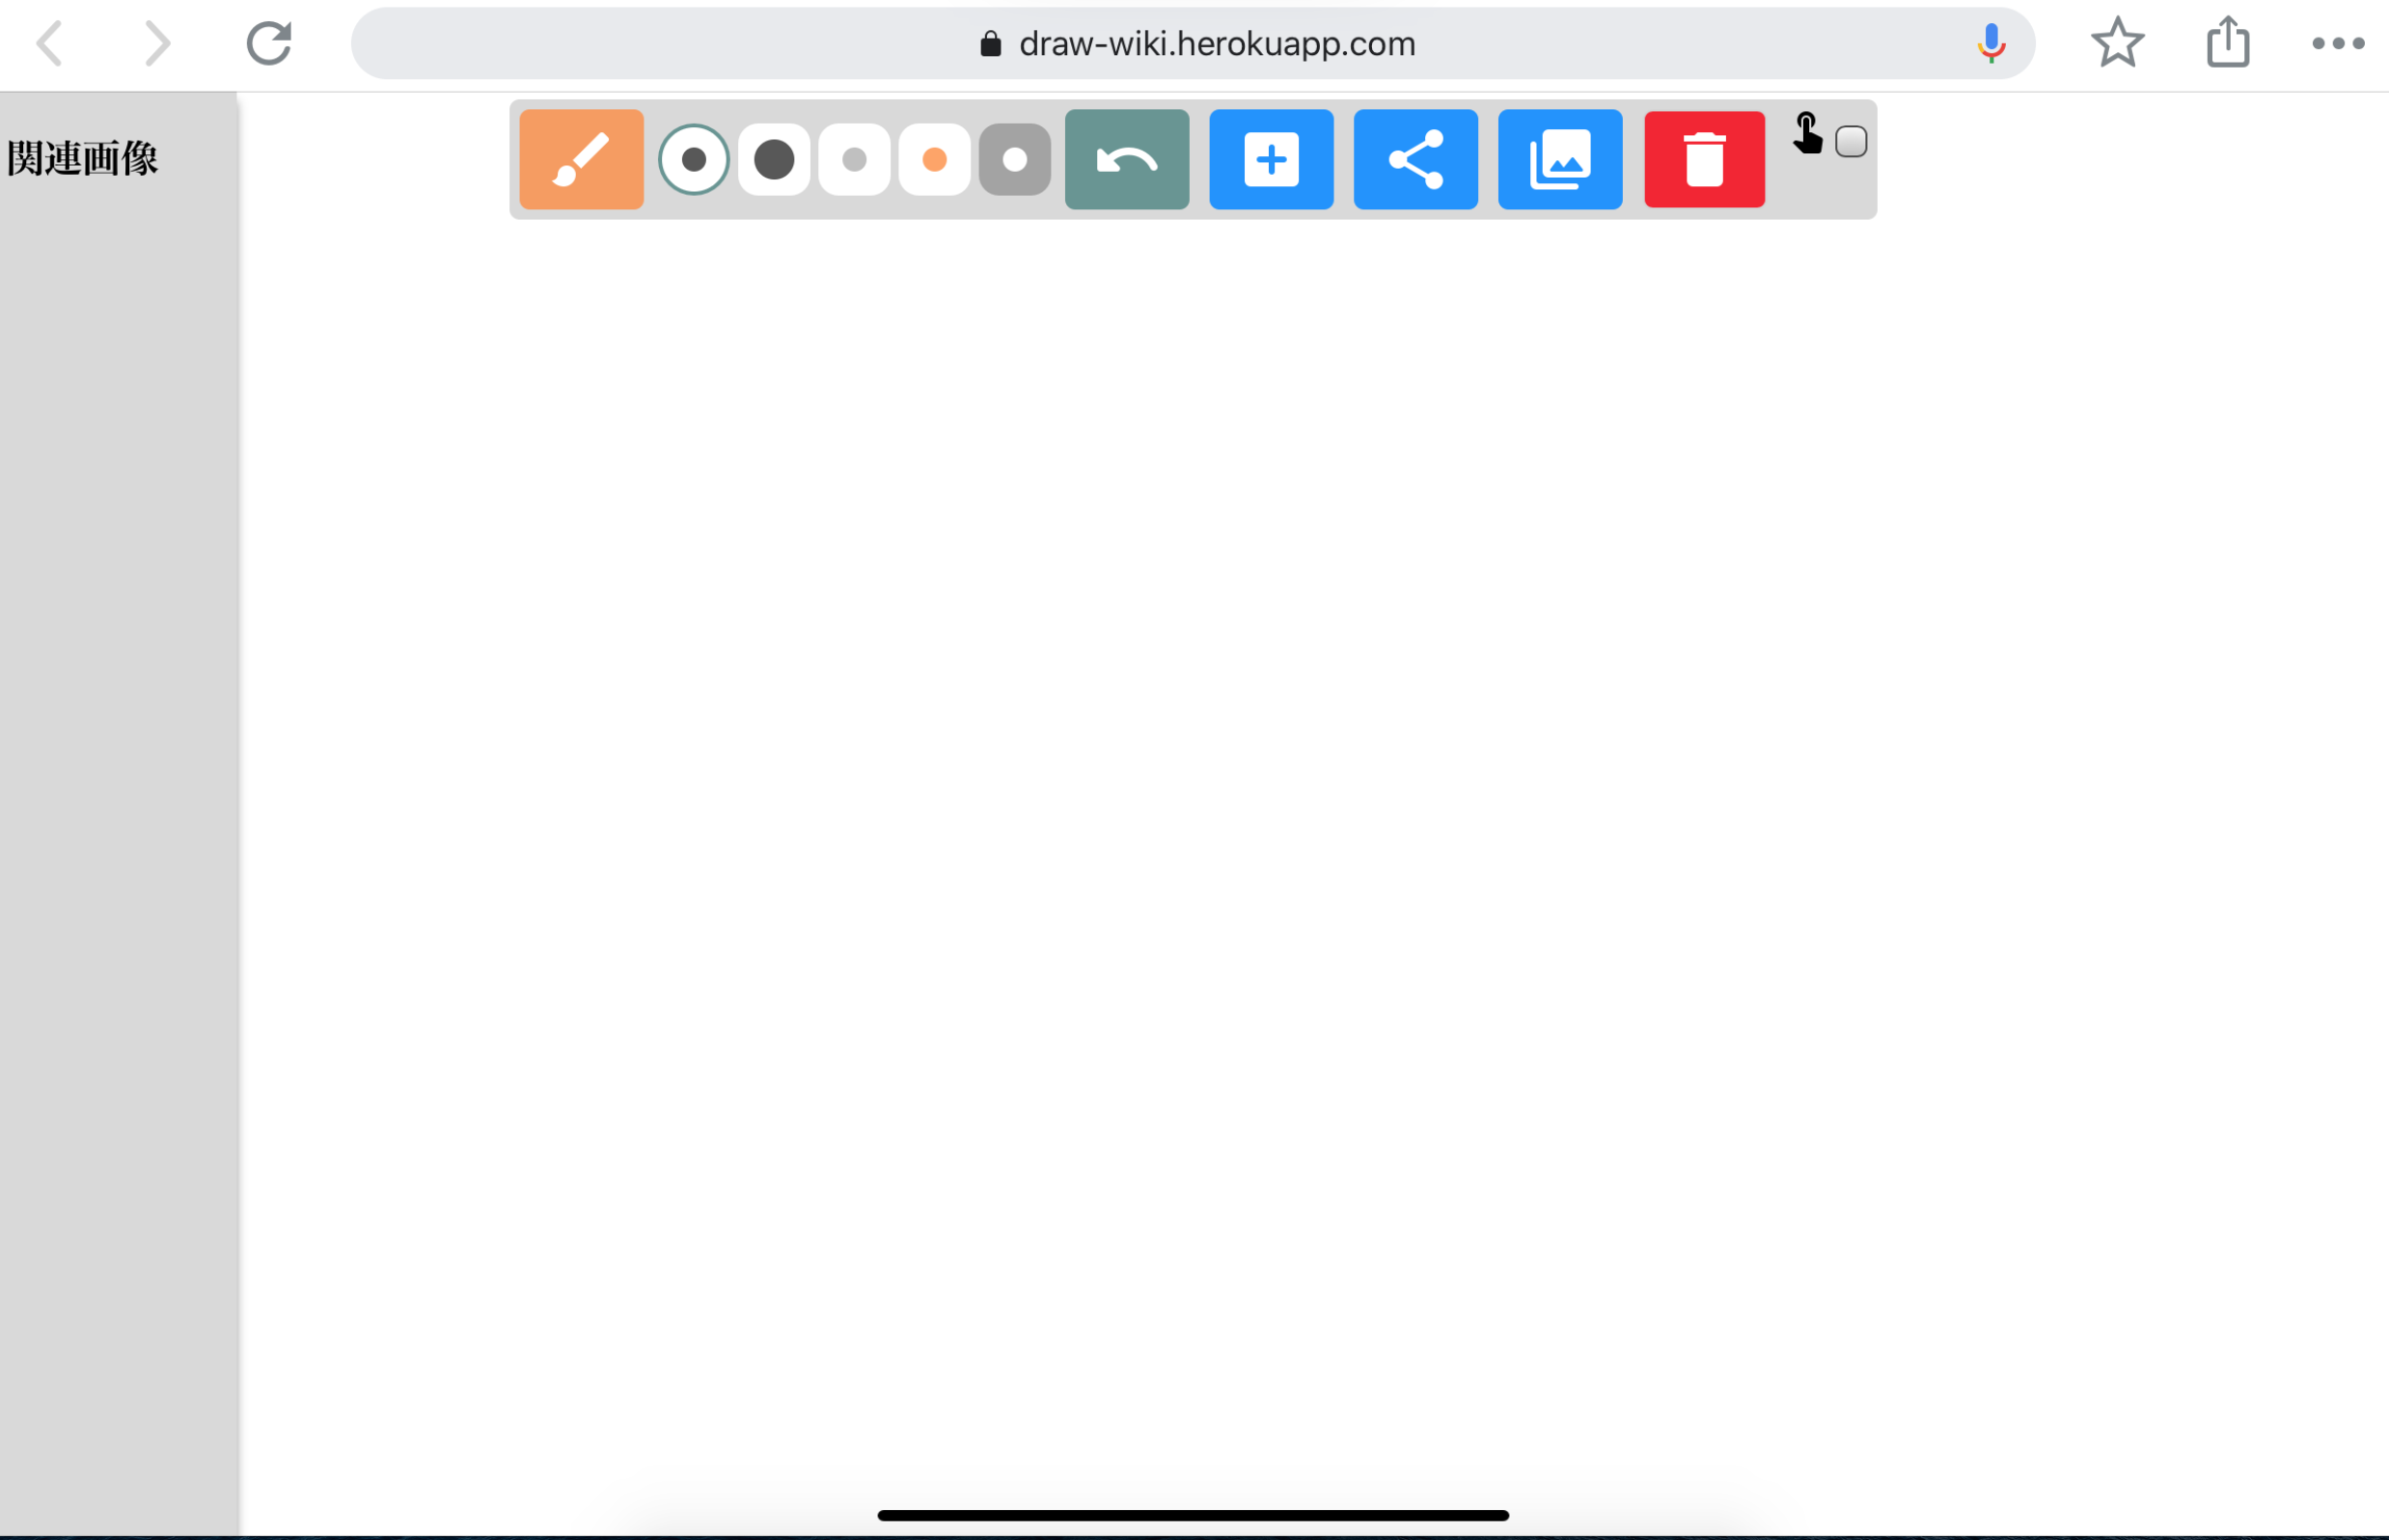
\includegraphics[width=50mm]{images/initialdrawwiki.png}} \end{center}
    \caption{Draw Wikiの初期画面}
    \label{drawwiki}
\end{figure}


\subsection{基本機能}
手書きデータを扱う既存のエディタと同様に、Draw WikiはUndo・Redoやオブジェクトの変形・移動等、計算機によって実現可能になった便利な編集支援機能を備えている。
これにより手軽に手書きメモ・イラストを作成することができる。

\subsection{特有の機能と使い方}
前章で述べた要件を満たすためにDraw Wikiは特有の機能を備えている。使い方とともに解説する。

\subsubsection{ハイパーリンク埋め込み機能}

\begin{figure}[htbp]
    \begin{center}
    {
\includegraphics[width=50mm]{images/testimage.png}} \end{center}
    \caption{ハイパーリンク埋め込み機能の操作画面}
    \label{hyperlinking}
\end{figure}

範囲選択ツールを用いてハイパーリンクを埋め込みたい要素を選択する。
画像リストから

\subsubsection{ハイパーイラストのインポート機能}

\begin{figure}[htbp]
    \begin{center}
    {
\includegraphics[width=50mm]{images/testimage.png}} \end{center}
    \caption{インポート機能の操作画面}
    \label{importing}
\end{figure}

過去に作成したハイパーイラストを一覧画面から選択し、現在編集中の画面にインポートすることができる。

\subsubsection{エキスポート・共有機能}

\begin{figure}[htbp]
    \begin{center}
    {
\includegraphics[width=50mm]{images/testimage.png}} \end{center}
    \caption{エキスポート機能の操作画面}
    \label{exporting}
\end{figure}

Draw Wikiで作成したハイパーイラストには各々に一意なURLが割り振られており、どこからでも参照することができる。
また範囲選択ツールを用いて一部の範囲のみ別個のハイパーイラストとしてエキスポートすることができる。
本体のSVGは

\subsubsection{ブラシプリセット}
その他の特徴としてブラシのプリセットが金箱らによるInteractive Sketch\cite{130004638060}に基づいている。
%ラーナビリティの観点から機能を


\begin{figure}[htbp]
    \begin{center}
    {
\includegraphics[width=50mm]{images/testimage.png}} \end{center}
    \caption{エキスポート機能の操作画面}
    \label{interacive}
\end{figure}